\documentclass[main.tex]{subfiles}
\begin{document}

\section{Neural Compositional Denotational Semantics for Question Answering} % 3pp
\label{sec:denotation-semantics}

\subsection{Introduction}
Compositionality is a mechanism by which the meanings of complex expressions are systematically determined from the meanings of their parts, and has been widely assumed in the study of both artificial and natural languages~\cite{montague-semantics} as a means for allowing speakers to generalize to understanding an infinite number of sentences. Popular neural network approaches to question answering use a restricted form of compositionality, typically encoding a sentence word-by-word, and then executing the complete sentence encoding against a knowledge source. Such models can fail to generalize from training data in surprising ways. Inspired by linguistic theories of compositional semantics, we instead build a latent tree of interpretable expressions over a sentence, recursively combining constituents using a small set of neural modules. Our model outperforms RNN encoders, particularly when test questions are longer than training questions.

Our approach resembles Montague semantics, in which a tree of interpretable expressions is built over the sentence, with nodes combined by a small set of composition functions. %The interpretation of the complete sentence corresponds to the answer to a question.
However, both the structure of the sentence and the composition functions are learned by end-to-end gradient descent. To achieve this, we define the parametric form of small set of composition modules, and then build a parse chart over each sentence subsuming all possible trees. Each node in the chart represents a span of text with a distribution over groundings (in terms of booleans and knowledge base nodes and edges), as well as a vector representing aspects of the meaning that have not yet been grounded. The representation for a node is built by taking a weighted sum over different ways of building the node (similar to \newcite{malliard-unsuptree-2017}). The trees induced by our model are linguistically plausible, in contrast to prior work on structure learning from semantic objectives~\cite{williams-latenttree-2018}.

% Typical neural approaches to grounded question answering first encode a question with a recurrent neural network (RNN), and then evaluate the encoding against an encoding of the knowledge source (for example, a knowledge graph or image) \citep{SantoroRBMPBL17}.
In contrast to classical approaches to compositionality, constituents of complex expressions are not given explicit interpretations in isolation.
For example, in \emph{Which cubes are large or green?}, an RNN encoder will not explicitly build an interpretation for the phrase \emph{large or green}.
We show that such approaches can generalize poorly when tested on more complex sentences than they were trained on.
%Such approaches have been shown weak generalization performance in some respects.
Our approach instead imposes independence assumptions that give a linguistically motivated inductive bias. In particular, it enforces that phrases are interpreted independently of surrounding words, allowing the model to generalize naturally to interpreting phrases in different contexts. In our model, \emph{large or green} will be represented as a particular set of entities in a knowledge graph, and be intersected with the set of entities represented by the \emph{cubes} node.

%Another perspective on our work is as a method for learning the layouts of Neural Module Networks (NMNs) \citep{andreas2016neural}.
Another perspective on our work is as a method for learning layouts of Neural Module Networks (NMNs)~\cite{nmn-2016}.
% Work on NMNs has focused on construction of the structure of the network, variously using rules, parsers and reinforcement learning \citep{Andreas2016LearningTC, Hu2017LearningTR}. Our end-to-end differentiable model jointly learns structures and modules by gradient descent.

Our model is a new combination of classical and neural methods, which maintains the interpretability and generalization behaviour of semantic parsing, while being end-to-end differentiable.

\begin{figure}[tb]
    \centering
    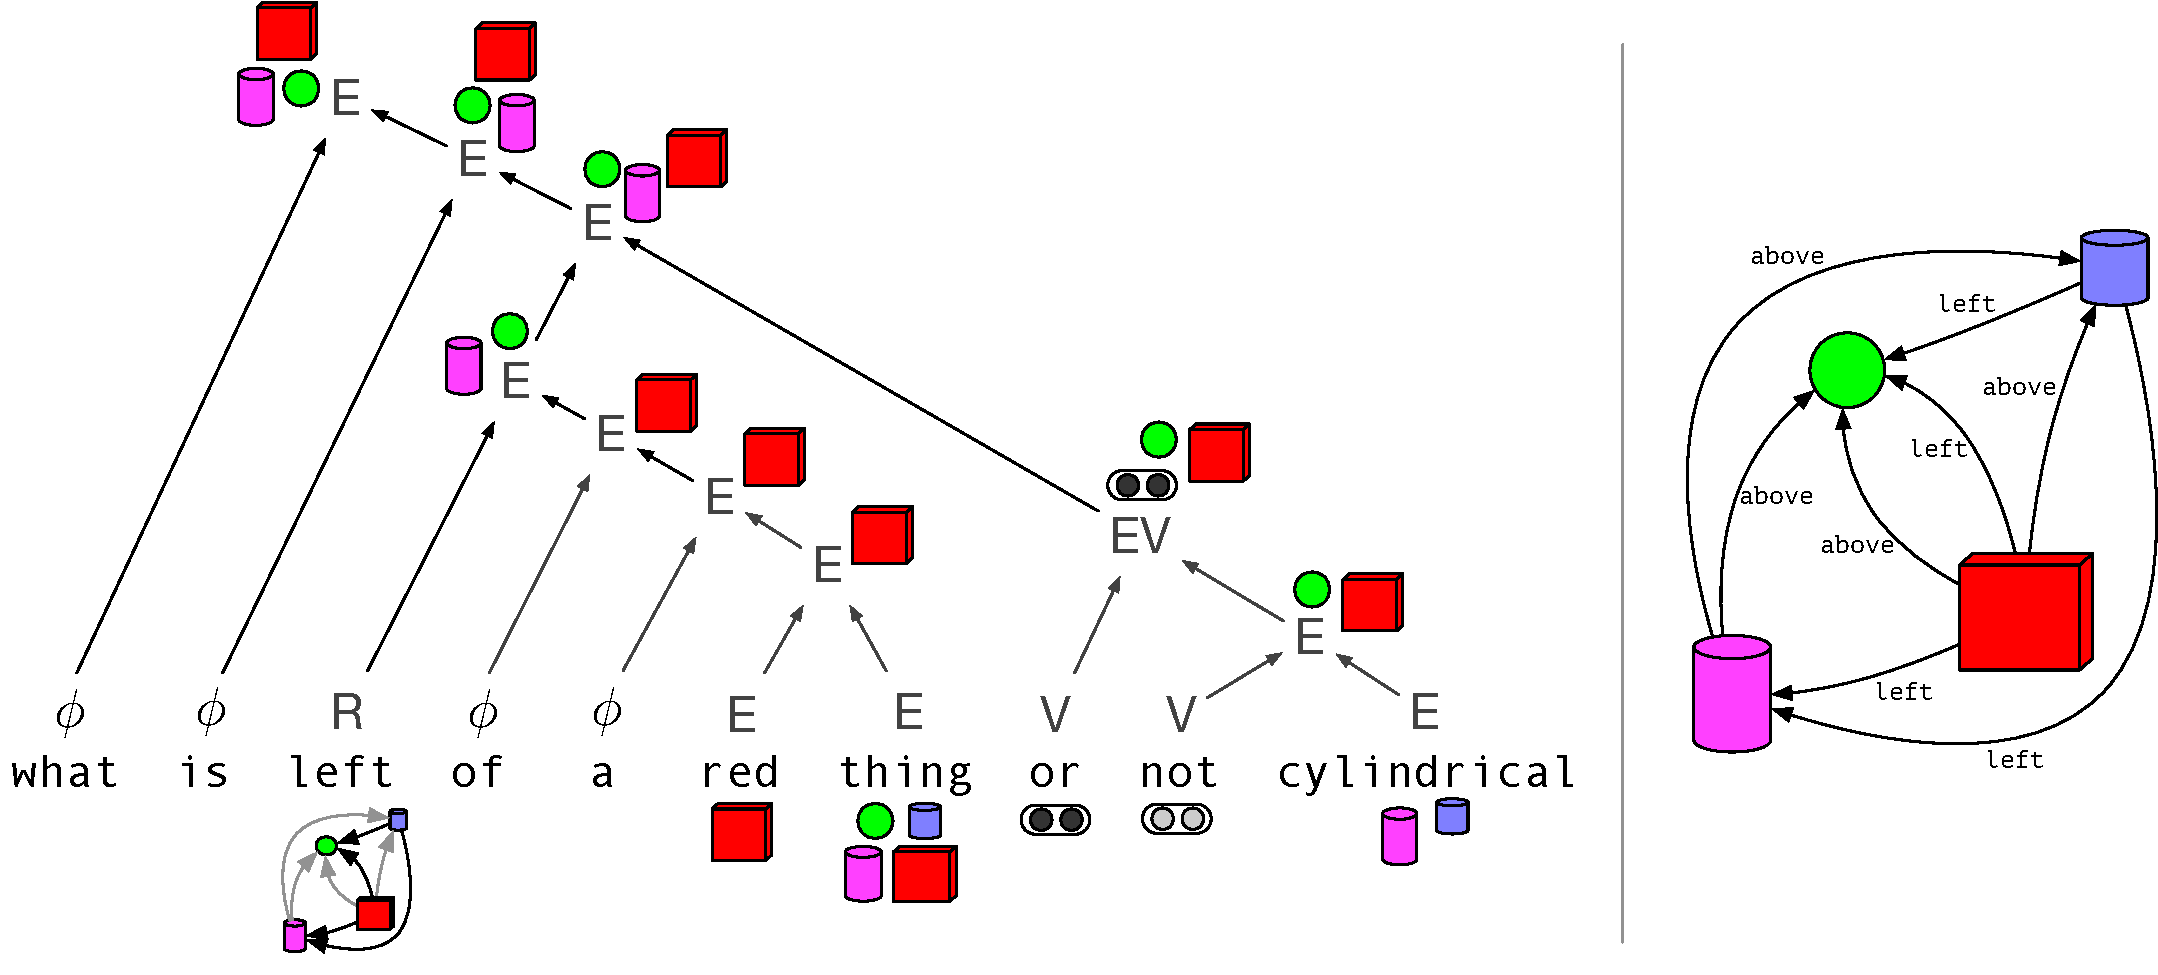
\includegraphics[width=\textwidth]{chapter-4/04-overview.pdf}
    \caption{{ A correct parse for a question given the knowledge graph on the right, using our model. We show the type for each node, and its denotation in terms of the knowledge graph. The words \emph{or} and \emph{not} are represented by vectors, which parameterize composition modules. The denotation for the complete question represents the answer to the question.
    Nodes here have types $E$ for sets of entities, $R$ for relations, $V$ for ungrounded vectors, $EV$ for a combination of entities and a vector, and $\phi$ for semantically vacuous nodes.
    While we show only one parse tree here, our model builds a parse chart subsuming all trees.} }
    \label{fig:04-overview}
\end{figure}

\biblio

\end{document}
